\section{Model selection}
\addcontentsline{toc}{section}{Model selection}
\label{sec:model_selection}

At first glance, one could think that the problems like the Happywhale challenge are generic multi-class classification task. This would mean that the model should be able to classify an input image of an individual correctly as just this individual. For tasks like this, the default approach is the following: \\
Feed the input image to some Convolutional Neural Network (CNN) architecture which outputs an embedding of this image. This embedding can then be flattened and fed into a Dense Layer which will output the predicted class. \cite{CNN-Courseware}

\begin{figure}[ht] 
        \centering 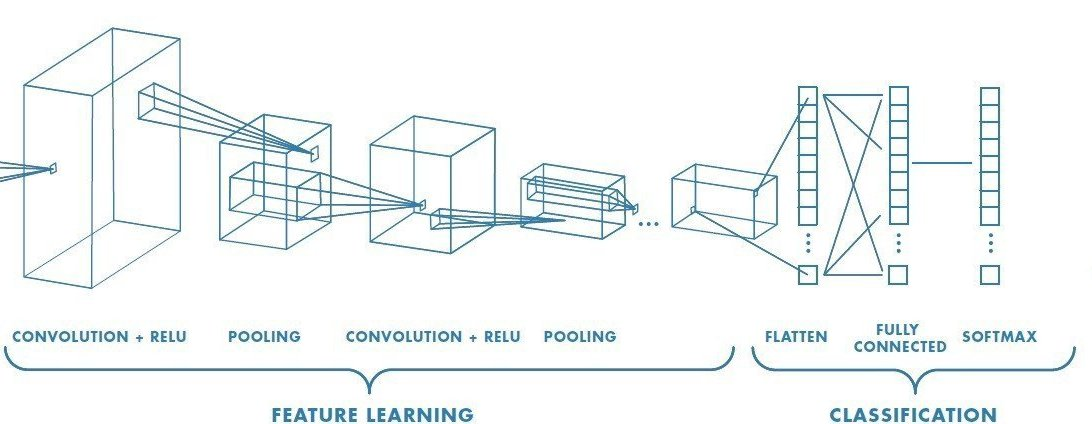
\includegraphics[width=1\columnwidth]{figures/cnn.jpeg}
        \caption{\label{fig:cnn_architecture_img} Vanilla image classification \protect\cite{cnn_architecture_img}.}
\end{figure}

\subsection{CNN architecture} \label{subsec:cnn}
As a first step of model selection we compare popular CNN architectures that we want to test. It is often a good idea to bet on architectures which already solidified their position on the grandstand of the machine learning domain of interest. Therefore we had a look at the most implemented models for image classification tasks. \\
Looking at this list we decide for a Residual Neural Network (ResNet), a Densely Connected Neural Network (DenseNet), an EfficientNet and an InceptionNet. \cite{paperswithcode}
All of these networks are notorious for being capable to classify images with very high accuracy while being somewhat computationally efficient (at least compared to other machine learning approaches). \\ 
Additionally, there are countless pre-trained models with easy access points available for these architectures. Especially the models pretrained on ImageNet \cite{deng2009imagenet}, one of the world's largest labeled image databases, are extremely powerful for image classification tasks and therefore of great interest to us. \\
We decided to try out the following architectures with pre-trained weights from ImageNet: ResNet50, ResNet50V2, DenseNet101, EfficientNet and InceptionNetV3. We also trained ResNet50 ourselves. More about that can be read in \hyperref[sec:softmax-model]{Softmax Model}.

\subsection{Softmax activation}
The activation function of the last Dense Layer in this pipeline is usually a Softmax function \shortcite{Training-Courseware}, which computes a probability distribution \(\sigma\) over the image membership for each class \(K\).
\[ \sigma(z_i) = \frac{e^{z_{i}}}{\sum_{j=1}^K e^{z_{j}}} \ \ \ for\ i=1, \dots, K \ \ \ \text{and} \ \ \ (z_1, ..., z_K) \in \mathbb{R}^K \]
\(K\) is determined by the constant number of neurons in the final Dense Layer.
Unfortunately, we are working with a dynamically changing number of classes - we do not know every individual whale in the ocean (let alone having images of them). \\
For now, this eliminates the Softmax activation function as a suitable approach to our task. \\

\subsection{Triplet loss}
Luckily, the domain of metric learning offers us an alternative approach which is more suitable for our problem: Triplet loss - originally presented in the FaceNet \cite{Schroff_2015} paper. \\
The goal of triplet loss is to learn an embedding space in which similar sample pairs stay close together and dissimilar ones are far apart. It does this by computing a distance between an anchor image \(a\) and a positive sample \(p\), as well as between \(a\) and a negative sample \(n\). \(a\) and \(p\) are different images of the same individual, while \(n\) is an image of a different individual.

\begin{figure}[ht] 
        \centering 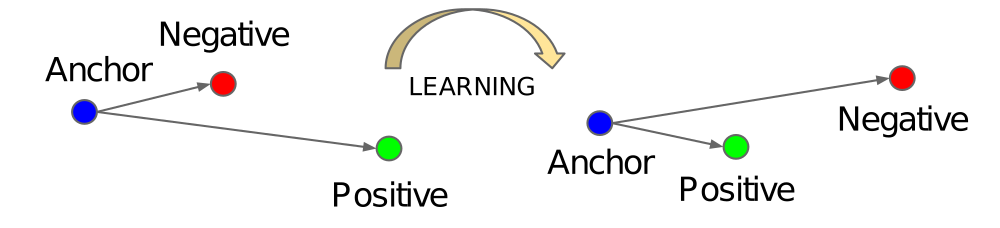
\includegraphics[width=1\columnwidth]{figures/triplet_loss.png}
        \caption{\label{fig:triplet_loss_img} Triplet loss visualized \protect\cite{Schroff_2015}.}
\end{figure}

\noindent The learning goal is then to minimize the distance between \(a\) and \(p\) and maximize the distance between \(a\) and \(n\) at the same time \cite{weng2021contrastive}. Triplet Loss for some triplet \((a,p,n)\) in the embedding space is defined as:
\[ \mathcal{L}_\text{triplet} = \max\left(0,d(a,p)-d(a,n) + \epsilon\right) \]
where \(d\) denotes the L2 norm (calculated from the euclidean distance between the embeddings) and the margin parameter \(\epsilon\) denotes the minimum offset between distances of \(d(a,n)\) and \(d(a,p)\). This prevents the the network of gaming the function and circumventing its actual intention. If there was no \(\epsilon\), the network could just map the complete data set onto the same point in the embedding. This would cause all distances and the loss to be 0. The margin ensures, that in this case, the loss would still be positive. \cite{hav4ik2021deepmetriclearning}\\

\subsubsection{Triplet Mining} \label{subsec:mining}
Of course, triplet loss is far from being a perfect method of choice as well. One of it's main limitations is that during one comparison only one negative example \(n\) is compared with the anchor \(a\). The disregard of all other \(n\) could lead to an embedding space where some dissimilar pairs are still in close proximity to each other - just because they were not compared against each other. \cite{Sohn_2016} \\
This is why, in order to train a triplet loss model successfully, one has to pay close attention to the composition of each triplet. If we want the model to learn something we should pick an \(n\) that is not obviously a different individual than \(a\). \\

\noindent To do this, we could choose a challenging \(n\) that is closer to the \(a\) than the positive sample \(p\).
\[ d(a,n) < d(a,p) \]
This is called \textit{hard triplet mining}. In theory, it should guarantee optimal learning success. However, it is prone to get stuck in local minima and the samples are rather hard to select from our data set. \\

\noindent An approach which tries to solve this is \textit{semi-hard triplet mining}. Here the triplets are chosen in a way, that \(n\) is not closer to \(a\) than \(p\), but the function still has a positive loss.
\[ d(a,p) < d(a,n) < d(a,p) + \epsilon \]
The distance between \(a\) and \(n\) is still in the range of margin \(\epsilon\). This way, the model can still learn but is more unlikely to end up in local minima. \\

\begin{figure}[ht] 
        \centering 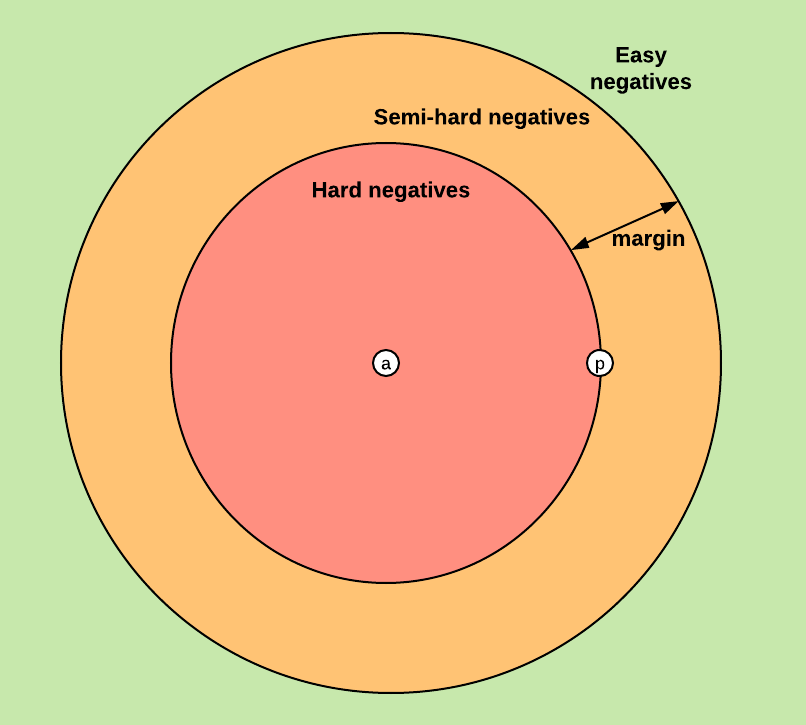
\includegraphics[width=1\columnwidth]{figures/triplet_mining.png}
        \caption{\label{fig:quellemussrein}Different kind of Negatives visualised \protect\cite{moindrot}.}
\end{figure}


\noindent We need to specify the triplet sampling process even further by choosing between \textit{offline} and \textit{online} triplet mining. \\
With \textit{offline mining}, the triplets are generated at the beginning of each epoch. The embeddings are computed on the training set and then only (semi-) hard triplets are selected. This technique is rather inefficient because we need to do a full pass on the training set for each epoch and update the triplets. \\
Doing \textit{online mining}, samples are produced for each batch of inputs. Within a batch of \(B\) examples we can find a maximum of \(B^3\) triplets. Many of these triplets are not of shape \((a,p,n)\) and are therefore not valid. Still, it does not require updating all samples offline and more samples are created for a single batch. This makes the approach way more efficient \cite{moindrot}.

\subsubsection{Shortcomings}
There still remain problems with the triplet loss function and contrastive learning approaches in general. \\
It is hard to guarantee that embeddings of the same individual will be pulled together in euclidean space (expansion problem). In addition, there is the so called sampling issue \cite{hav4ik2021deepmetriclearning}: Online triplet mining is hard to implement for very unbalanced data sets like our Happywhale data set. \\
There are modern alternatives to triplet loss such as Cos- and ArcFace, which are based on angular distance and margin. They (partially) solve the above problems but we nevertheless wanted to try out vanilla triplet loss and see how far we will come with this approach. Since our paper should also be of some educational value and explain the concepts well to other students, triplet loss is also more suitable because it is less advanced and needs fewer prerequisites to understand. \\
Because of the mentioned advantages in \hyperref[subsec:mining]{Triplet mining}, we also decided to implement online semi-hard triplet mining. \\
There is still one disadvantage of triplet loss which we did not talk about up until now: Evaluation of training progress is computationally expensive. As we want to evaluate the usefulness of the different \hyperref[subsec:cnn]{CNN architectures}, we need to compute an evaluation metric (i.e. accuracy) on the validation set after each training epoch. To do this, the embedding of every image from the validation set needs to be compared to all embeddings of the training set. This means there have to be many point-wise distance calculations in a high dimensional euclidean space calculated. To be specific, we need to do $37598 *  4177$ computations in a $256$-dimensional embedding space for each epoch. Furthermore, the convergence time for triplet loss models is said to be rather high. \\
Doing this for more multiple hyperparameter settings for each architecture is not feasible with our computational resources. Is there a cheaper workaround?

\subsection{Combining Softmax and Triplet Loss}
We already found out that the Softmax activation function is not useful for our final model but maybe we could still utilize it for some architecture comparison. Computing accuracy of a Softmax based model is a breeze compared to models based on contrastive loss. \\
We can imagine that an architecture that performs well over a finite-class classification task using Softmax is also likely to perform well for a classification problem with a dynamical number of classes like Happywhale. So why not try this out? \\
Our approach will now look like the this: \\
We will train the said models with a fixed size Softmax Dense layer at the end on the different (fixed) whale species. During this training process, we evaluate their performance on the validation set, taking accuracy and convergence speed into account. After training is finished, we compare their performance on the test set and select the most robust and promising architecture for our final triplet loss model.\\

\noindent The final model will essentially be a Siamese Network which is composed of 2 identical CNN architectures that share their weights. The according inputs are the sample pairs \((a,p)\) and \((a,n)\) which are then projected into the embedding space. As explained earlier, the triplet loss then should ensure reasonable euclidean distances between the embedding pairs.
